\documentclass[problem]{mcs}

\begin{pcomments}
  \pcomment{PS_figure_eight_countable}
  \pcomment{zabel 10/10/17}
\end{pcomments}

\pkeywords{
  sets
  countable
  rationals
  figure_eight
}

\newcommand\Circle{\operatorname{Circ}}
\newcommand\FE{\operatorname{FigEight}}
\newcommand\bR{\reals}
\newcommand\bQ{\rationals}

\begin{problem}
  For a point $p\in\bR^2$ in the plane\footnote{The notation $\bR^2$ is shorthand for $\bR\times\bR$} and a positive real number $r > 0$, let $\Circle(p,r)$ be (the border of) the circle with center $p$ and radius $r$:
  $$\Circle(p,r)\eqdef \{v\in\bR^2 \mid |v - p| = r\}.$$
  Two circles $C,C' \subset \bR^2$ \emph{intersect} when they have a point (or more) in common, i.e., $C\cap C' \ne \emptyset$; they are \emph{disjoint} otherwise. For example, two tangent circles intersect each other, but two circles with one entirely enclosed within the other are disjoint. 

  \bparts
  \ppart Find a simple bijection from the real numbers $\reals$ to the \emph{positive} real numbers $\reals^+$, and conclude that $\reals^+$ is uncountable.

  \begin{solution}
    The function $f(x) \eqdef e^x$ works. We already know that $\reals$ is uncountable, so this bijection proves that $\reals^+$ is also uncountable.
  \end{solution}
  
  \ppart Describe a total injection $f$ from the positive real numbers into the set of circles, with the property that whenever $s \ne s'$, circles $f(s)$ and $f(s')$ don't intersect each other. This shows that it is possible to find uncountably many circles in the plane, no two of which intersect each other.
  
  \begin{solution}
    The function $f(s)\eqdef \Circle((0,0), s)$ works. For a proof by contradiction, suppose $s\ne s'$ but $v\in f(s) \cap f(s')$. Because $v$ is in circle $f(s)$ it follows that $|v| = s$, but for the same reasons, $v\in f(s')$ implies $|v| = {s'}$. This contradicts $s\ne s'$, so these two circles must indeed be disjoint.
  \end{solution}

  \ppart
  If $p\ne q$ are two distinct points in the plane, define the \term{figure eight} shape $\FE(p,q)$ as the union of two equally-sized tangent circles centered at $p$ and $q$:
  \begin{equation*}
    \FE(p,q) \eqdef \Circle(p,r) \cup \Circle(q,r), \qquad \text{where $r = |p-q|/2$}.
  \end{equation*}
  In the remainder of this problem we'll answer the following question: can uncountably many disjoint figure eights fit in the plane, just like for circles? We'll show the answer is ``NO, only countably many''.

  To start out, let $E = \FE(p,q)$ be a figure eight as above. It is possible to choose a point $v\in\bQ^2$ with rational coordinates enclosed by one of $E$'s circles, and another point $w\in\bQ^2$ with rational coordinates enclosed by $E$'s other circle; in this case, we call $(v,w)$ a \emph{mark} for $E$.

  % If $v$ and $w$ are two points in the plane, we say that $(v,w)$ is a \term{mark} for $E$ if $E$'s two circles enclose $v$ and $w$, respectively: $|v - p| < r \QAND |w - q| < r$. Show that it is possible to find a mark $(v,w)$ for $E$ where $v$'s and $w$'s coordinates are \emph{rational} numbers. \emph{Hint}: Any disk contains a square.

  % \begin{solution}
  %   The square with side-length $r$ and center $p = (x,y)$ is enclosed by $\Circle(p,r)$, as may easily be verified geometrically. We may find a rational number $a\in [x-r/2, x+r/2]$ and a rational number $b \in[y - r/2, y+r/2]$, so that rational point $v=(a,b)$ lies in this square and is thus enclosed within $\Circle(p,r)$. A rational point $w$ enclosed by $\Circle(q,r)$ may similarly be found, making $(v,w)$ a mark for $E$ with rational coordinates.
  % \end{solution}

  \label{partNoMarkDuplicates}
  If $E = \FE(p,q)$ and $E' = \FE(p',q')$ are disjoint figure eights, prove that no $(v,w)$ can be a mark for both $E$ and $E'$. \emph{Hint}: There are two cases to consider, as in Figure~\ref{fig:disjoint-figure-eights}.

  \begin{figure}[hbt]
    \centering
    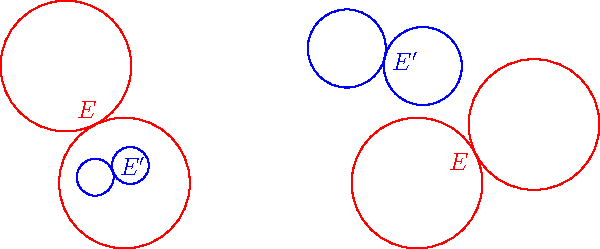
\includegraphics[height=1.5in]{disjoint-figure-eights}
    \caption{The two configurations of a pair of disjoint figure eights: one of $E$ or $E'$ encloses the other (left), or neither encloses the other (right).}
    \label{fig:disjoint-figure-eights}
  \end{figure}
  
  \begin{solution}
    Suppose $(v,w)$ marks both $E$ and $E'$. Since $E$ and $E'$ are disjoint, one of them encloses the other in one of its circles, or neither encloses the other.

    In the first case, without loss of generality, we may assume that $E$ encloses $E'$. Because $(v,w)$ marks $E'$, both $v$ and $w$ are enclosed by $E'$ and thus by the the same circle of $E$. So neither $v$ nor $w$ lies within the \emph{other} circle of $E$, meaning $(v,w)$ cannot mark $E$.

    The second case, where neither $E$ nor $E'$ marks the other, is similar: since $(v,w)$ marks $E'$, both points must be enclosed within $E'$ and thus cannot be enclosed by $E$.

    In either case, the assumption that $(v,w)$ marks both $E$ and $E'$ cannot hold, as desired.
  \end{solution}
  
  \ppart Assume $A$ is any set of figure eights where no two of $A$'s figure eights intersect. We can define a total function $g: A \to (\bQ^2)^2$ by picking a rational mark $g(E)$ for each figure eight $E\in A$, as described above. Prove that $g$ is injective, and use this to prove that $A$ must be countable.

  You may use the fact that if $Y$ and $Z$ are countable sets, then $Y\times Z$ is also countable (Problem~\bref{MQ_product_of_countables}).

  \begin{solution}
    It follows directly from Part~\ref{partNoMarkDuplicates} that $g$ is injective: any two figure eights $E$ and $E'$ in $A$ are disjoint (by assumption), and we showed above that this means marks $f(E)$ and $f(E')$ for them cannot be equal. So $A \inj (\bQ^2)^2$. To conclude that $A$ is countable, it thus suffices to show that $(\bQ^2)^2$ itself is countable. This follows by two applications of Problem~\bref{MQ_product_of_countables}: we know $\bQ$ is countable, so $\bQ\times \bQ = \bQ^2$ is countable, and thus $(\bQ^2)\times (\bQ^2)$ is countable.
  \end{solution}
  
  \eparts
\end{problem}

\endinput
